\documentclass{report}

\usepackage[a4paper, total={6in, 8in}, margin=1in,footskip=0.25in]{geometry} \usepackage{amsmath, amsthm, amssymb, booktabs, chemfig, graphicx, float, pgfplots, setspace, siunitx, tabularray} \usepackage{tabularray} \usepackage[hidelinks]{hyperref}

\setlength{\parindent}{0pt}
\setlength{\parskip}{0.8em}

\pgfplotsset{compat=1.18}

\graphicspath{ {.././Images/} }

\title{\Huge Year 12 Physics - Module 6}
\author{L. Cheung}

\tolerance=1
\emergencystretch=\maxdimen
\hyphenpenalty=10000
\hbadness=10000

\begin{document}

	\maketitle
	\newpage

\section*{Practical Investigation 6.1 - A current-carrying conductor in a uniform magnetic field, force versus current}

	\textbf{Aim:} To investigate the relationship between force and current for a current carrying conductor in a magnetic field.

	\subsection*{Materials}
		\begin{itemize}
			\item Current balance
			\item Connecting wires
			\item Ammeter
			\item Rheostat
			\item Power supply
			\item Ruler
		\end{itemize}
	
	\subsection*{Variables}
	
		\begin{table}[htbp]
			\centering
			\setstretch{1.25}
			\begin{tabular}{l|l}
				Independent	& Current \\
				Dependent	& Mass required to balance \\
				Control		& Temperature, voltage, length inside solenoid, magnetic field strength
			\end{tabular}
		\end{table}
	
	\subsection*{Risk Assessment}
	
		\begin{table}[htbp]
			\centering
			\setstretch{1.25}
			\begin{tabular}{l|l}
				\textbf{Hazard}			& \textbf{Precaution} \\ \hline
				Electrocution		& Turn off power supply while modifying circuit \\
				Damage to equipment	& Keep devices away from solenoid
			\end{tabular}
		\end{table}

	\subsection*{Method}
		\begin{enumerate}
			\item Set up the current balance
			\item With no current flowing, level the current balance
			\item Position the solenoid around the current balance
			\item Connect a power supply and ammeter to the current balance. A second power supply should be connected to the solenoid.
			\item Increase the current into the balance and re-level it using masses.
			\item Record the mass required to level the balance depending on the current flow
		\end{enumerate}
	
	\subsection*{Results}
		\begin{table}[htbp]
			\centering
			\setstretch{1.25}
			\begin{tabular}{p{2.5cm}|p{2.5cm}|p{2.5cm}}
				\textbf{Current}	& \textbf{Mass}	& \textbf{Force} \\ \hline
				0.5 	& 0.060	& 0.00059	\\
				1	& 0.072	& 0.00071	\\
				1.5	& 0.084	& 0.00082	\\
				2	& 0.096	& 0.00094	\\
				2.5	& 0.11	& 0.0011	\\
				3	& 0.12	& 0.0012	\\
				3.5	& 0.12	& 0.0012
			\end{tabular}
		\end{table}

		\begin{align*}
			B &= \frac{\mu_0 N I}{L} \\
			  &= \frac{\mu_0 \times 700 \times I}{0.15}
		\end{align*}
		\begin{align*}
			F &= BIl \sin{\theta} \\
			\frac{F}{I} &= Bl = \text{gradient} \\
				    &= B \times 0.025
		\end{align*}

	\subsection*{Data and Analysis}

		\begin{enumerate}
			\item \textbf{When investigating the relationship between force and current, what angle should the wire along the end of the current balance make with the magnetic field? Why?}

				The wire at the end of the current balance should be perpendicular to the magnetic field so that the maximum force is generated, ie. $\sin{\theta}=1$

			\item \textbf{Why can the effect of the connection wires along the length of the current balance be ignored?}
				
				The connection along the length of the current is parallel to the magnetic field and therefore experiences no force. Therefore, it does not affect the result.

			\item \textbf{Calculate the force corresponding to each measurement of mass and record it in the corresponding column of the results. How is force calculated?}
				
				$$F_B = mg$$

			\item \textbf{Determine the equation of the relationship between the force and current of the data}

				Force is directly proportional to current. From the graph, $F = 2.48 \times 10^{-4} I$
		
		\end{enumerate}
	
	\subsection*{Conclusion}

		\begin{enumerate}
			\item \textbf{What is the nature of the relationship between these two variables?}

				Force and current have a linear relationship.

			\item \textbf{What does this say about how changes in the current will affect the force acting on a wire that is in a magnetic field?}

				Force is directly proportional to current.

			\item \textbf{What is the significance of the gradient of the graph? How reliable was the value you found}

				The gradient of the graph shows the relationship between force and current. The data was very reliable.

		\end{enumerate}

\newpage

\section*{Practical Investigation 6.2 - Parallel wires, quantitative data analysis} \label{24/02/2025}

	\textbf{Aim:} To quantitatively analyse the way two parallel current-carrying conductors interact.

	\subsection*{Data and Analysis}
	
		\begin{enumerate}
			\item \textbf{What will be the ratio of the current in the top wire to that in the bottom wire?}
				\subitem The ratio is one to one.

			\item \textbf{Will the wires attract or repel? Explain your answer.}
				\subitem Consider the bottom rod. By right hand grip rule, the magnetic field above the rod is into the page. Due to the motor effect, the top wire experiences an upwards force. Similarly, the top wire has a magnetic field into the page that exerts a downward force on the bottom wire. Therefore, the two wires are repelled from each other.

			\item \textbf{The cables are now brought toward each other and the force per unit length between them is measured. Assuming that the power supply is supplying a constant 10A of current, complete the following table for the variation in distance.}

				\begin{table}[htbp]
					\centering
					\setstretch{1.25}
					\begin{tabular}{p{5cm}|p{5cm}}
							Distance $d$ (cm)	& $\frac{F_B}{l}$ (Nm$^{-1}$)	\\ \hline
							30			& $6.67 \times 10^{-7}$		\\
							25			& $8.00 \times 10^{-7}$		\\
							20			& $1.00 \times 10^{-6}$ 	\\
							15			& $1.33 \times 10^{-6}$ 	\\
							10			& $2.00 \times 10^{-6}$ 	\\
							5			& $4.00 \times 10^{-6}$ 	\\
							1			& $2.00 \times 10^{-5}$
					\end{tabular}
				\end{table}

			\begin{figure}
				\centering
				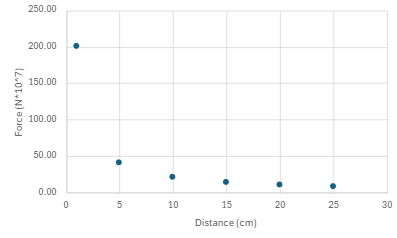
\includegraphics[width=15cm]{prac 6.2.png}
				\caption{Force over Distance graph}
			\end{figure}

			\item \textbf{At what distance apart would the force due to the magnetic field around each wire be sufficient to balance the mass of the top wire? Assume that the wires are straight and the lower wire is unable to move away.}
			
				\begin{align*}
					m &= 1540 \times 0.001 \\
					  &= 1.54 \text{kg}
				\end{align*}

				\begin{align*}
					F_G &= ma \\
					    &= 1.54 \times 9.8 \\
					    &= 15.1 \text{N}
				\end{align*}
				
				\begin{align*}
					F_B &= \frac{\mu_0 I}{2 \pi r} \times l \times I \\
					    &= \frac{\mu_0 I^2 l}{2 \pi r} \\
					r &= \frac{\mu_0 I^2 l}{2 \pi F_B}
				\end{align*}

				\begin{center}
					Let $F_B = F_G$
				\end{center}
				
				\begin{align*}
					r &= \frac{\mu_0 I^2 l}{2 \pi F_G} \\
					  &= 0.133 \times 10^{-6} \text{ m}
				\end{align*}

			\item \textbf{The cable is designed to support a maximum continuous current of 110A. If the cable were carrying this current, at what distance would the force between the wires balance the mass of the top wire?}

				\begin{align*}
					r &= \frac{\mu_0 I^2 l}{2 \pi F_G} \\
					  &= 1.60 \times 10^{-4}
				\end{align*}

			\item \textbf{If the force experienced by the top wire is exactly balancing the force due to gravity, would the force experienced by the bottom wire be larger, the same, or small? Explain your answer.}

				The net force of the bottom wire would be greater. The top wire is not fixed in place and still has no acceleration, therefore has a net force of 0. The bottom wire experiences a repulsion force and the force of gravity in the same direction, therefore has a greater net force.
		\end{enumerate}

\end{document}
